\input{preamble}

Commands are entered in the following field.

\begin{center}
\begin{tikzpicture}
\node at (0,0) {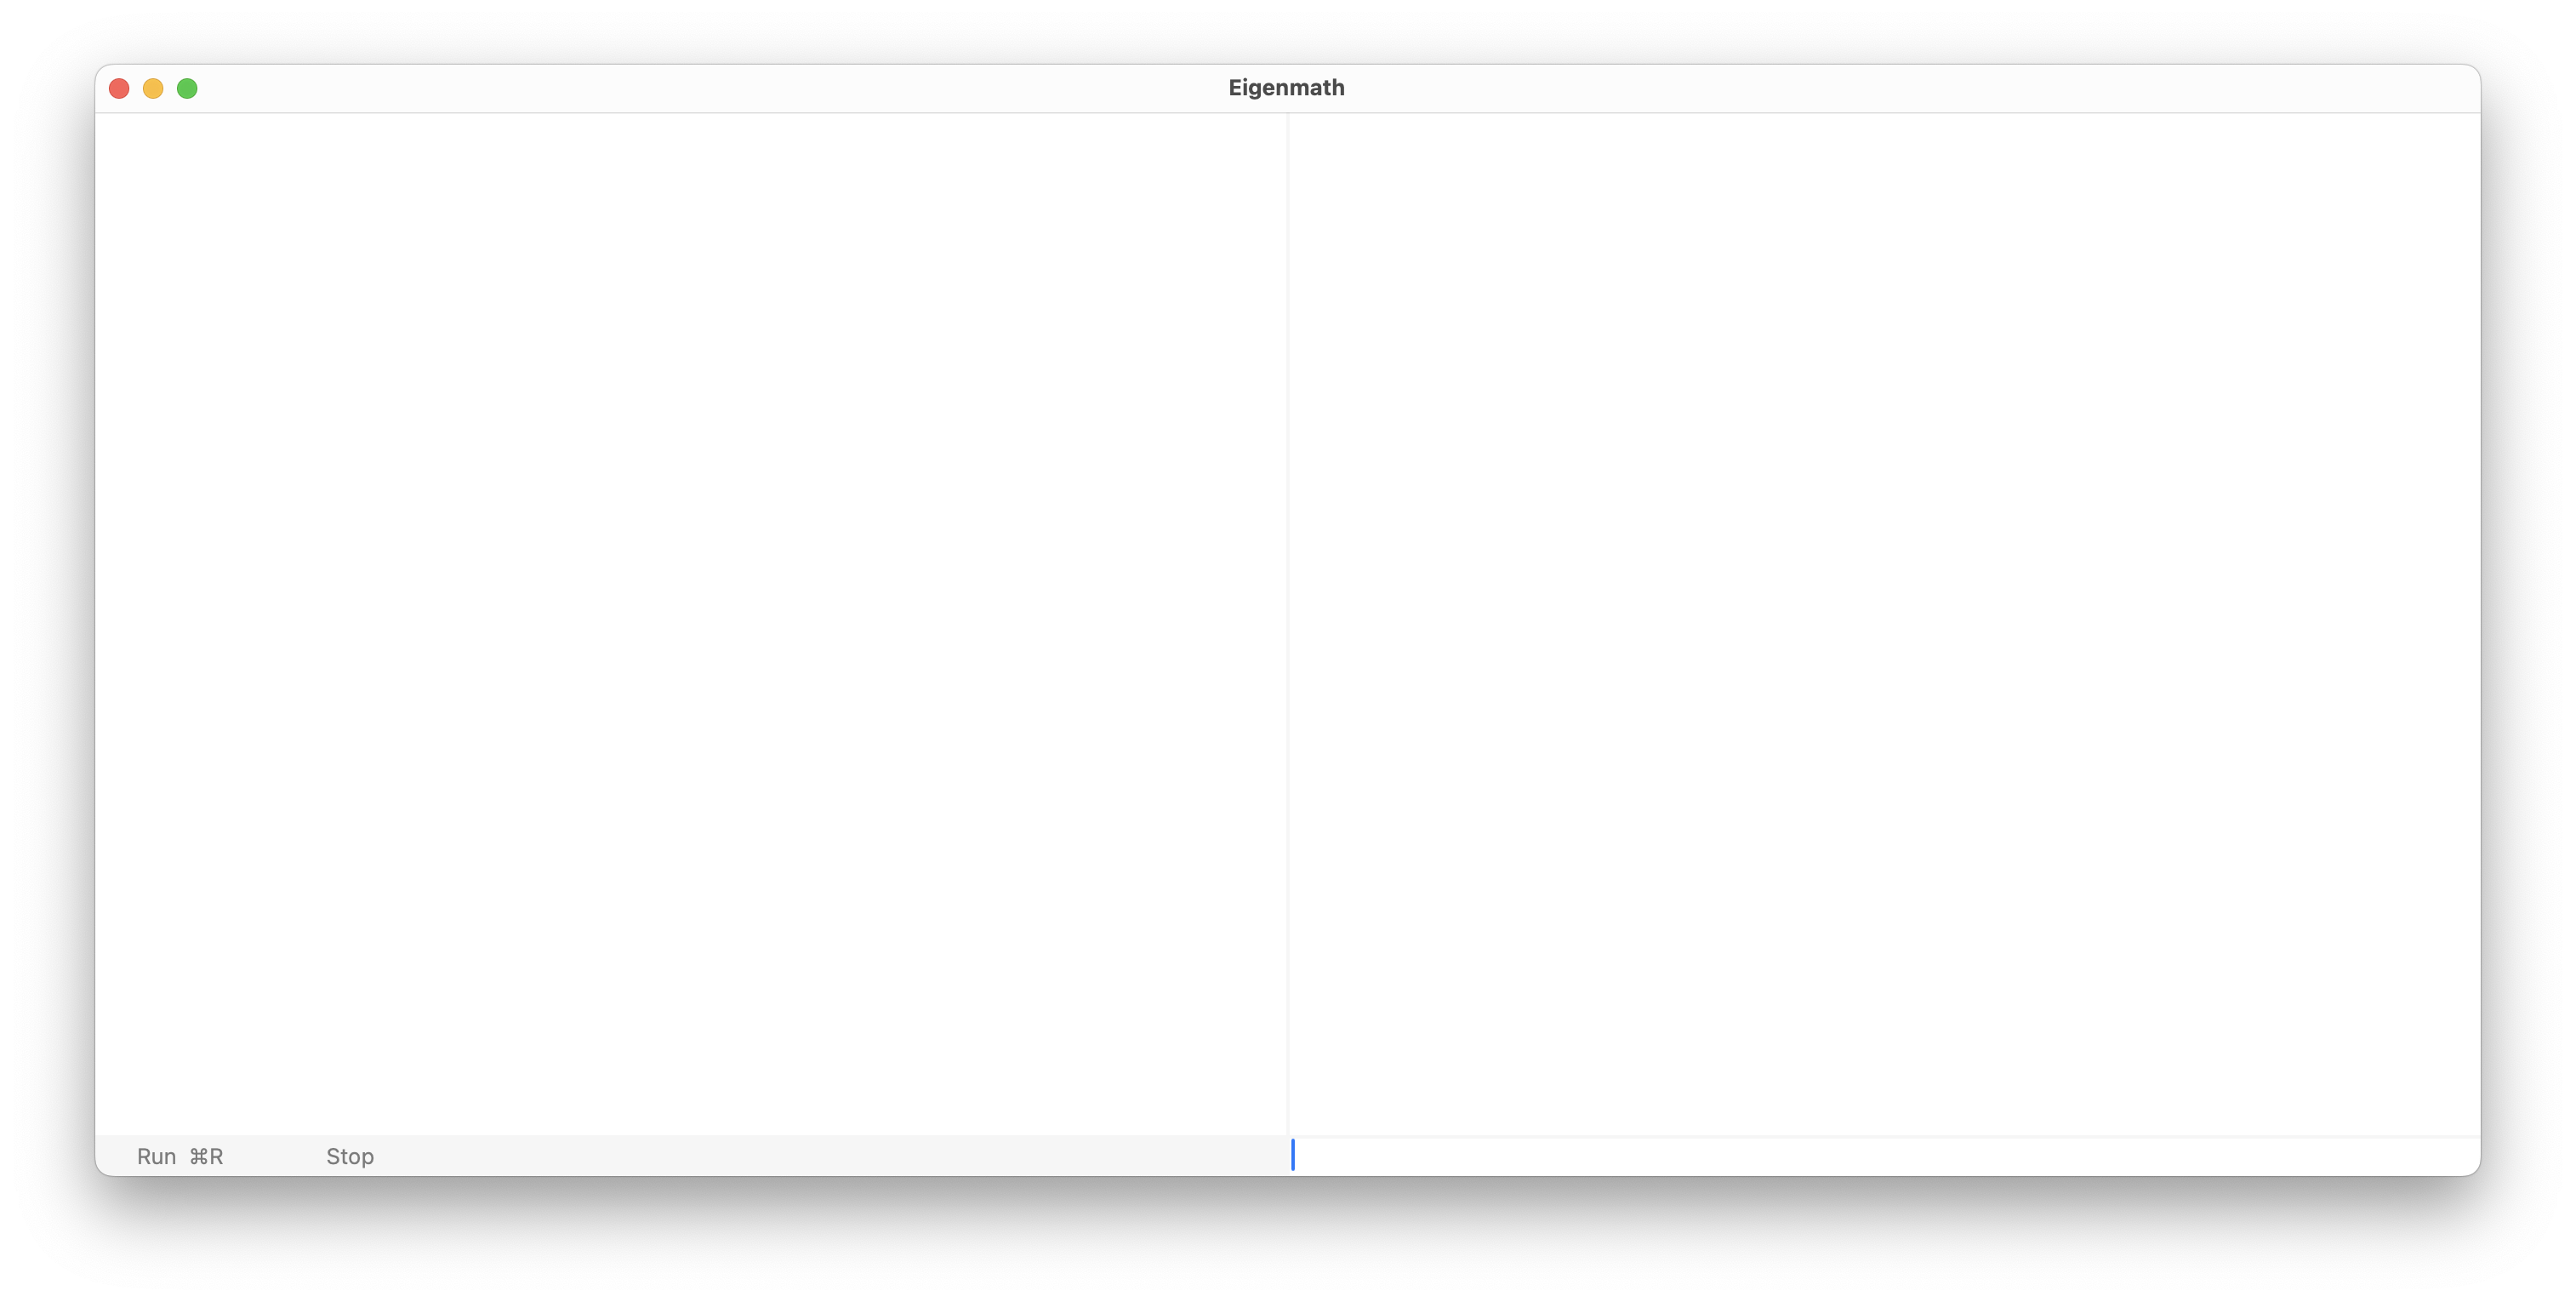
\includegraphics[scale=0.25]{screenshot.png}};
\draw[red,thick] (3,-2.6) ellipse (3.5cm and 0.5cm);
\end{tikzpicture}
\end{center}

Multiple commands can be put together in a script.
Scripts are run by clicking the Run button.

\begin{center}
\begin{tikzpicture}
\node at (0,0) {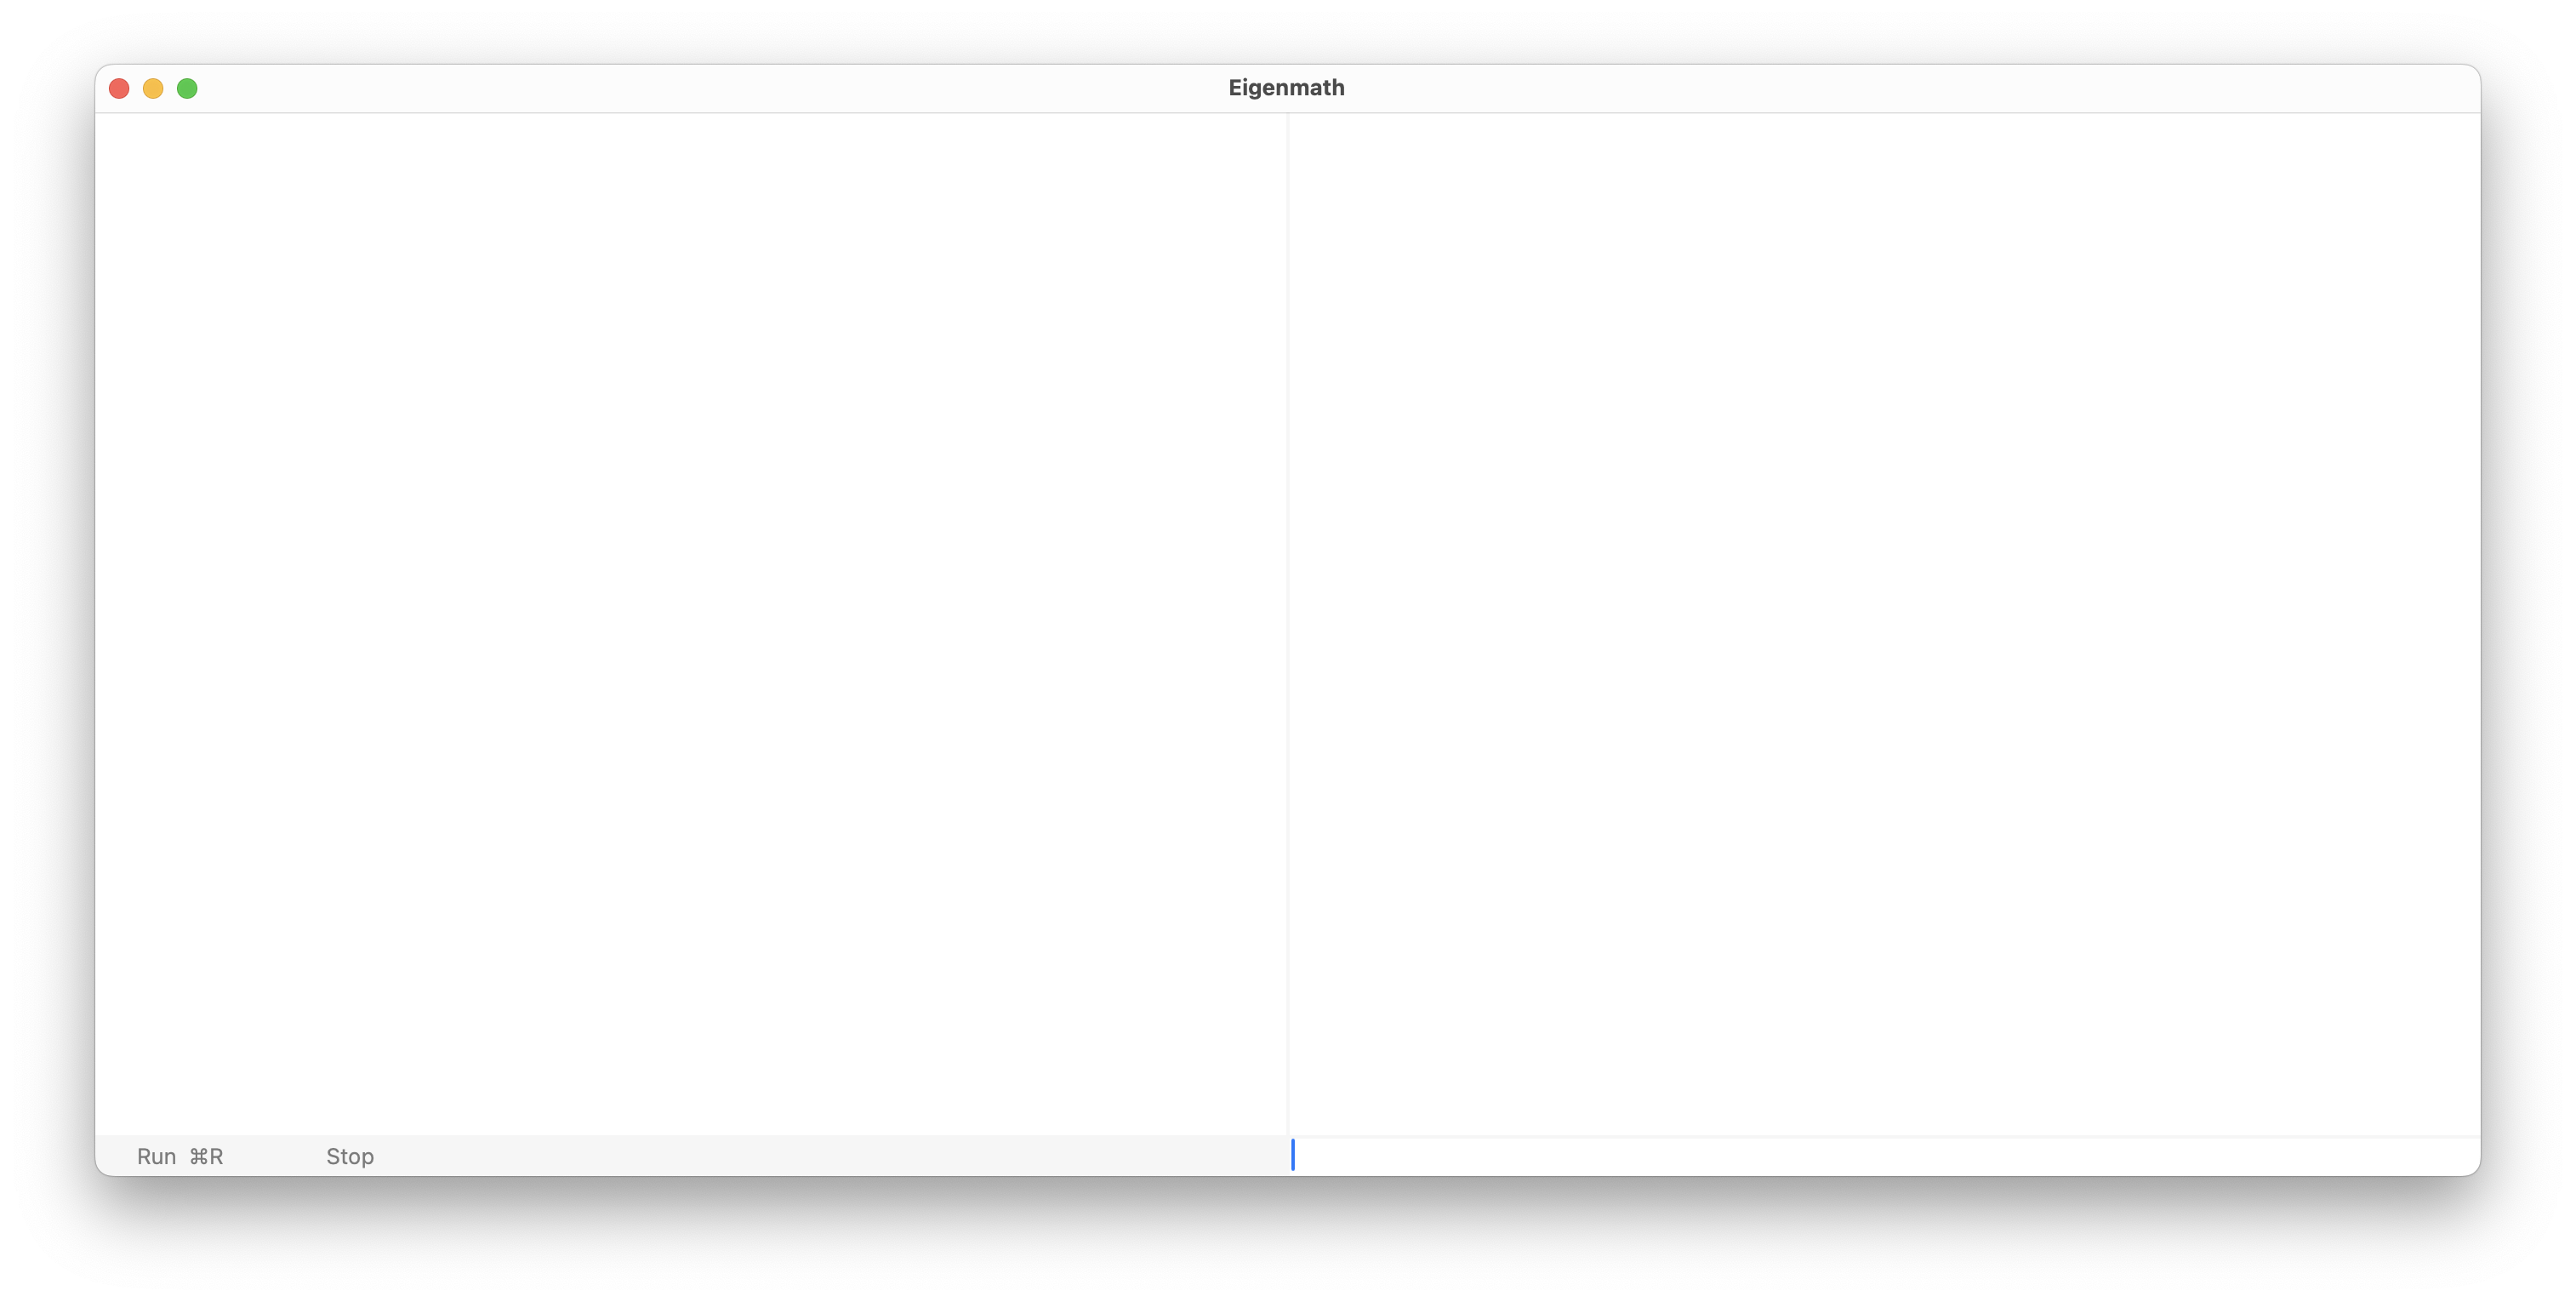
\includegraphics[scale=0.25]{screenshot.png}};
\draw (-3,0) node {Scripts go here};
\end{tikzpicture}
\end{center}

After a script runs, all of the results are available in command mode.

\iffalse
\bigskip
To print or copy results, click in the result field.
Then press \cmd$\,$P to print, \cmd$\,$C to copy to the clipboard.
\fi

\bigskip
Note: Times New Roman and Times New Roman Italic fonts need
to be the standard Mac fonts that include special symbols and Greek letters.
See the following link for correcting font problems.

\bigskip
{\footnotesize\verb$support.apple.com/guide/font-book/restore-fonts-that-came-with-your-mac-fb34862/mac$}

\end{document}
